\documentclass[fleqn]{report}
\usepackage[utf8]{inputenc}
\usepackage{graphicx}
\usepackage{fancyhdr}
\usepackage{amsmath}
\usepackage{xcolor}
\usepackage{subfigure}
\usepackage{pdfpages}
\usepackage{hyperref}
\usepackage{xepersian}
%In order to write persian in latex, with "texlive" distro installed, two additional packages are needed: texlive-xetex & texlive-lang-arabic

\settextfont[BoldFont={XB Zar bold.ttf}]{XB Zar.ttf}

\begin{document}

%Title Page
\begin{titlepage}
    \begin{center}
        
\includegraphics{sharif.png}\\
        \vspace{1cm}    \textbf{\LARGE   \lr{Speech Enhancement and Denoising}}\\
        \vspace{1cm}  \textbf{\Large  پروژه پایانی درس پردازش گفتار}\\
        \vspace{1cm}    \textbf{\large  دانشکده مهندسی کامپیوتر}\\
        \vspace{0.5cm}  \textbf{\large  استاد: دکتر صامتی}\\
        \vspace{0.5cm}  \textbf{\large  بهار ۱۴۰۳}\\
        \vspace{0.5cm}  \noindent\rule{8cm}{0.4pt}\\
        \vspace{2cm}    \textbf{\large بهار بهزادی‌پور \ \   ۴۰۲۲۰۷۱۵۵}\\
        \vspace{0.5cm}    \textbf{\large مهتا فطرت \ \   ۴۰۲۲۱۲۲۲۵}\\
        \vspace{2cm}    \textbf{\large \href{https://github.com/MahtaFetrat/Speech-Enhancement-and-Denoisnig}{مخزن پروژه}}\\
    \end{center}
\end{titlepage}

\tableofcontents

%Header & Footer
\pagestyle{fancy}
\fancyhf{}
\rhead{
\includegraphics[scale=0.1]{sharif.png} پردازش گفتار}
\lhead{Speech Enhancement and Denoising}
\rfoot{Page \thepage}

%Document Body

\chapter{مقدمه}
بهبود کیفیت گفتار و رفع نویز آن همواره مورد توجه بوده‌است و جزء معدود مسائل حوزه‌ی پردازش گفتار است که می‌توان گفت هنوز کاملا حل‌شده تلقی نمی‌شو و جای پیشرفت دارد.
با این حال، مدل‌ها و ابزار‌های بسیاری برای بهبود گفتار زبان انگلیسی وجود دارد که از کیفیت مطلوبی نیز برخوردار هستند.
در این میان، زبان فارسی نسبت له تکنولوژی‌های اخیر در این زمینه جای پیشرفت زیادی دارد.
بررسی‌های اولیه نشان می‌دهد که مدل بهبود گفتاری که برای زبان فارسی مناسب‌سازی شده باشد در حال حاضر وجود ندارد.
در این پروژه ما در تلاش هستیم تا وضعیت ابزار‌های حاضر را برای بهبود گفتار فارسی بررسی کنیم و بتوانیم در راه بهبود آن‌ها گام‌های موثری برداریم.

\section{شرح مسئله}
بهبود گفتار \lr{(Speech Enhancement)}  حذف نویز \lr{(Denoising)} به  فرآیندهایی اطلاق میشود که کیفیت و وضوح سیگنال گفتار را بهبود میبخشند و نویزهای پس زمینه را کاهش میدهند. این مسئله در کاربردهای مختلفی از جمله سیستم های تشخیص گفتار، ارتباطات تلفنی، و کمک به افراد با مشکلات شنوایی اهمیت دارد. در زبان فارسی، به دلیل تفاوت های صوتی و ساختاری با دیگر زبان ها، نیاز به تحقیق و توسعه ویژه ای در این زمینه وجود دارد.

\section{رویکردها}
در مورد مسئله‌ی بهبود گفتار و رفع نویز مانند بسیاری از مسائل دیگر در حوزه‌ی گفتار، دو رویکرد کلی وجود دارد.
اولین رویکرد مربوط به روش‌های 
rule-based می‌باشد.
این روش‌ها عموما مبتنی بر تکنیک‌های پردازش سیگنال می‌باشند و به مشاهده‌ی نمونه‌ی گفتار‌های تمیز و نویزی وابسته نیستند.
رویکرد دوم اما
مبتنی بر شبکه‌های 
عصبی می‌باشد.
در این روش‌ها، با داشتن یک معماری مناسب و تعداد زیادی از نمونه‌های ورودی و خروجی مطلوب، مدل می‌آموزد که تسک بهبود گفتار را انجام دهد.
در این پروژه، ما هر دوی این روش‌ها را بررسی می‌کنیم و راه‌حل‌هایی بر اساس هر یک ارائه می‌دهیم.

\section{چالش‌ها}
همانطور که برای سایر راه‌حل‌های مبتنی بر شبکه‌های عصبی  
چالش داده مطرح است، در این‌جا هم با این مشکل مواجه هستیم.
درواقع تهیه‌ی دادگانی طبیعی متشکل از زوج‌های تمیز و نویزی یک گفتار واحد، امری دشوار و زمان‌بر است. 
به همین جهت غالبا شاهد دیتاست‌هایی هستیم که به صورت اتوماتیک generate شده‌اند.
در ادامه به این موضوع بیشتر پرداخته می‌شود.

\section{اهداف و دستاورد‌های این پروژه}
در این پروژه ما ابتدا روش‌های موجود را برای زبان فارسی ارزیابی کردیم و امکان خاص‌سازی آن‌ها برای زبان فارسی را بررسی نمودیم.
سپس از بین روش‌های موجود، سعی در بهبود برخی از این روش‌ها به کمک تکنیک‌هایی چون fine-tuning داشتیم.
همچنین به عنوان یک جایگزین، ابزاری rule-based برای بهبود گفتار فارسی نیز ارائه دادیم که حتی بدون داده‌های آموزش نیز قابل استفاده است.
لازم به ذکر است که در این پروژه، دو نوع دیتاست نیز برای تسک \lr{Speech Enhancement and Denoising} برای زبان فارسی ارائه می‌شود که \lr{to the best of our knowledge} اولین دیتاست‌های این زبان در این تسک،‌ حتی از نوع ساختگی آن می‌باشد.

\chapter{مرور کارهای پیشین}
در این بخش به بررسی برخی از مهم‌ترین راه‌حل‌های موجود برای \lr{Speech Enhancement and Denoising} می‌پردازیم.

\section{Metricgan}

تفاوت بین تابع هزینه‌ای که برای آموزش مدل بهبود گفتار استفاده می‌شود و درک شنیداری انسان معمولاً باعث می‌شود که کیفیت گفتار بهبود یافته رضایت‌بخش نباشد. معیارهای ارزیابی عینی که درک انسان را در نظر می‌گیرند می‌توانند به عنوان پلی برای کاهش این فاصله عمل کنند. مدل MetricGAN که قبلاً پیشنهاد شده بود، برای بهینه‌سازی معیارهای عینی با اتصال معیار به یک تفکیک‌کننده طراحی شده بود. از آنجا که در طول آموزش تنها به امتیازات توابع ارزیابی هدف نیاز است، معیارها حتی می‌توانند غیرقابل تفکیک باشند. در این مطالعه، ما MetricGAN+ را پیشنهاد می‌کنیم که در آن سه تکنیک آموزشی که دانش حوزه پردازش گفتار را در خود دارند، پیشنهاد شده است. با این تکنیک‌ها، نتایج آزمایشی بر روی مجموعه داده VoiceBank-DEMAND نشان می‌دهد که MetricGAN+ می‌تواند امتیاز PESQ را نسبت به مدل قبلی MetricGAN به میزان 0.3 افزایش دهد و به نتایج برتر دست یابد (امتیاز PESQ = 3.15).
ایده اصلی MetricGAN شبیه‌سازی رفتار یک تابع ارزیابی هدف (مثلاً تابع PESQ) با یک شبکه عصبی (مثلاً Quality-Net [20]) است. تابع ارزیابی جانشین از امتیازات خام یاد گرفته می‌شود و تابع ارزیابی هدف را به عنوان یک جعبه سیاه در نظر می‌گیرد. هنگامی که ارزیابی جانشین آموزش داده شد، می‌توان از آن به عنوان یک تابع هزینه برای مدل بهبود گفتار استفاده کرد. متأسفانه، یک جانشین ایستا به راحتی توسط نمونه‌های تقلبی فریب می‌خورد.
برای بهبود عملکرد چارچوب MetricGAN، برخی تکنیک‌های پیشرفته یادگیری پیشنهاد شده‌اند. در طی این تحقیق، عواملی که به‌طور قابل‌توجهی بر عملکرد یا کارایی آموزش تأثیر می‌گذارند نیز بررسی می‌شوند. بهبود MetricGAN+ عمدتاً از طریق سه تغییر زیر حاصل می‌شود.
\begin{enumerate}
    \item یادگیری امتیازات معیار برای گفتار نویزی
    \item نمونه‌ها از بافر بازپخش تجربه
    \item تابع سیگموید قابل یادگیری برای تخمین ماسک
\end{enumerate}

\begin{figure}[h]

    \centering
    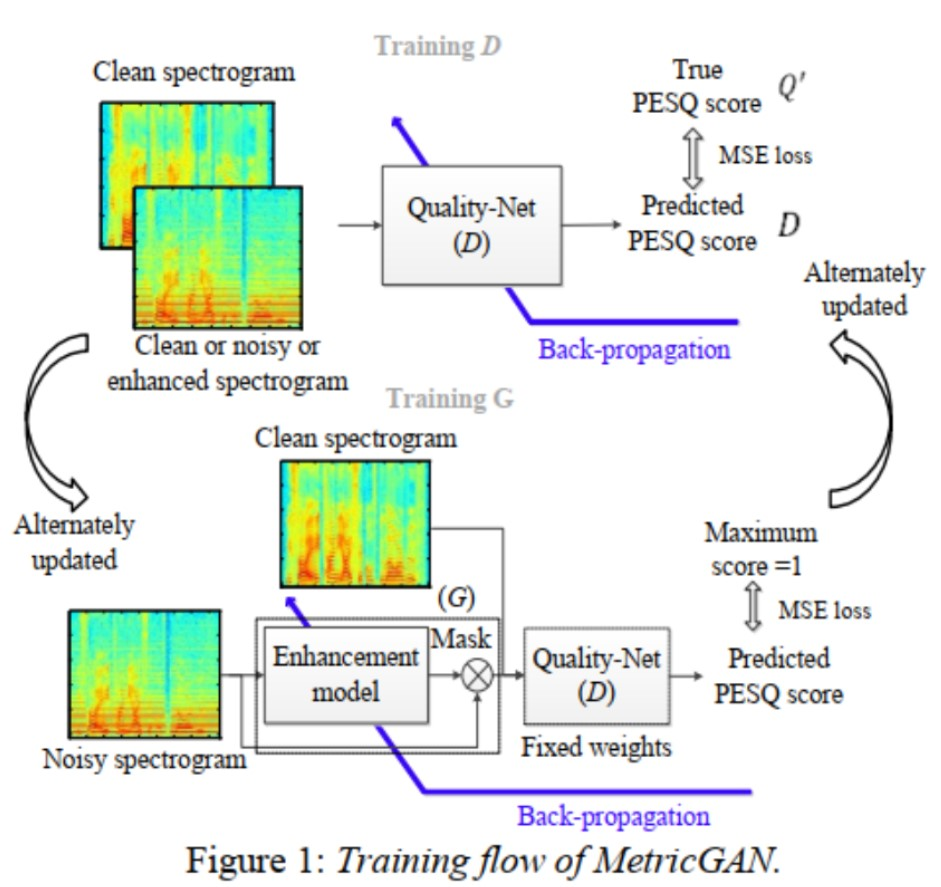
\includegraphics[width=.6\textwidth, keepaspectratio]{images/metricgan.jpg}
    
    \caption{آموزش metricgan}
    \label{fig:metricgan-training}
\end{figure}

در این مطالعه، چندین تکنیک برای بهبود عملکرد چارچوب MetricGAN پیشنهاد کردیم. ما متوجه شدیم که شامل کردن گفتار نویزی برای آموزش تفکیک‌کننده و استفاده از سیگموید قابل یادگیری، مفیدترین تکنیک‌ها هستند. MetricGAN+ ما نتایج پیشرفته‌ای را بر روی مجموعه داده‌های VoiceBank-DEMAND به‌دست می‌آورد و امتیازهای PESQ می‌تواند به ترتیب 0.3 و 0.45 نسبت به MetricGAN و BLSTM (MSE) افزایش یابد.

\section{Diff-TTS}
با وجود اینکه مدل‌های تبدیل متن به گفتار (TTS) عصبی توجه زیادی را جلب کرده و در تولید گفتار شبیه به انسان موفق بوده‌اند، هنوز جای پیشرفت‌هایی برای طبیعی‌تر و کارآمدتر کردن آن‌ها وجود دارد. در این کار، ما یک مدل TTS غیر اتورگرسیو جدید به نام Diff-TTS پیشنهاد می‌کنیم که به تولید گفتار با کیفیت بالا و کارآمدی بالا دست می‌یابد. با توجه به متن، Diff-TTS از یک چارچوب دیفیوژن نویززدایی برای تبدیل سیگنال نویز به طیف‌نگار مل از طریق مراحل زمان دیفیوژن استفاده می‌کند. به‌منظور یادگیری توزیع طیف‌نگار مل با شرط متن، ما یک روش بهینه‌سازی مبتنی بر احتمال برای TTS ارائه می‌دهیم. علاوه بر این، برای افزایش سرعت استنتاج، ما از روش نمونه‌برداری تسریع‌شده استفاده می‌کنیم که به Diff-TTS امکان می‌دهد تا موج‌نگاشت‌های خام را به‌طور بسیار سریع‌تری تولید کند بدون اینکه کیفیت ادراکی به‌طور قابل توجهی کاهش یابد. از طریق آزمایش‌ها، تایید کردیم که Diff-TTS با یک GPU NVIDIA 2080Ti به‌طور 28 برابر سریع‌تر از زمان واقعی تولید می‌کند.
دیف-TTS توزیع نویز را به توزیع مل-اسپکتروگرام متناظر با متن داده شده تبدیل می‌کند. همان‌طور که در شکل 1 نشان داده شده است، مل-اسپکتروگرام به تدریج با نویز گوسی تخریب شده و به متغیرهای نهان تبدیل می‌شود. این فرآیند، فرآیند انتشار نامیده می‌شود.

\begin{figure}[h]

    \centering
    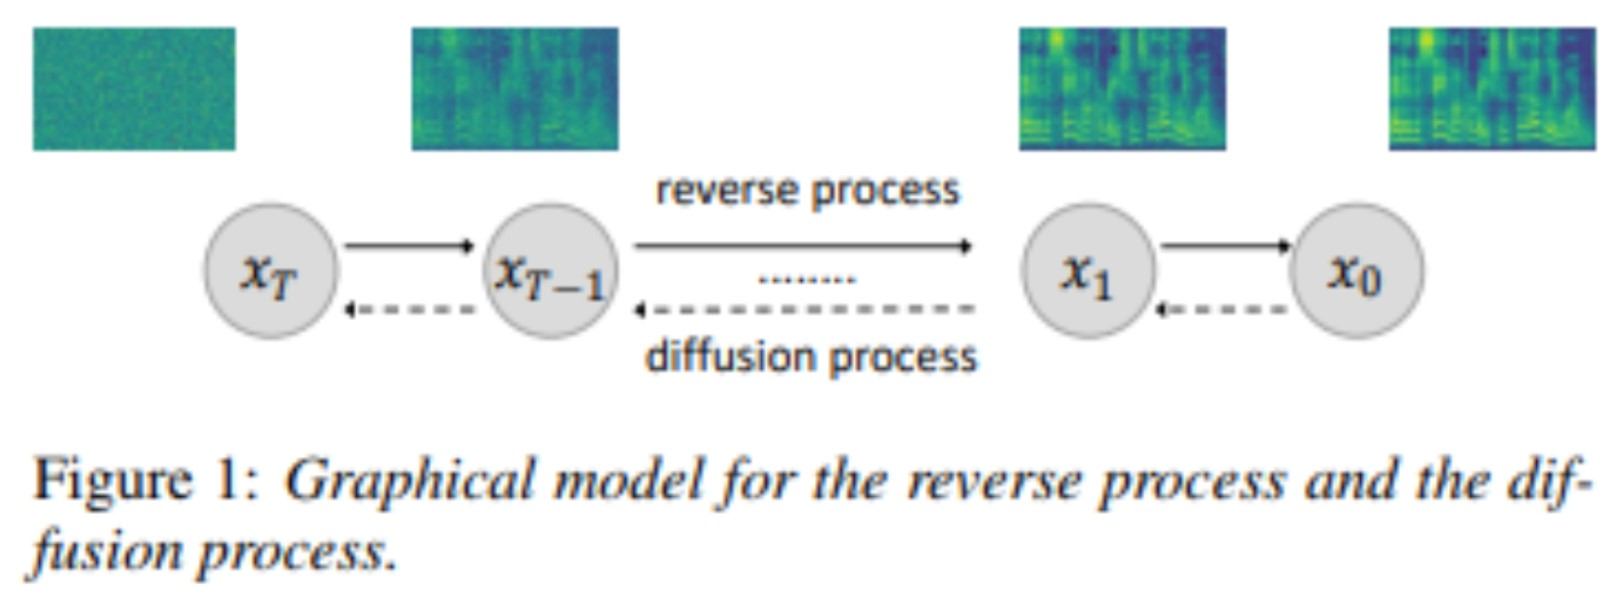
\includegraphics[width=.6\textwidth, keepaspectratio]{images/diffusion.jpg}
    
    \caption{فرایند diffusion}
    \label{fig:diffusion}
\end{figure}

فرض کنید x1, . . . , xT یک دنباله از متغیرها با ابعاد یکسان باشد که در آن t = 0, 1, . . . , T شاخصی برای مراحل زمانی انتشار است. سپس، فرآیند انتشار مل-اسپکتروگرام x0 را از طریق یک زنجیره انتقال‌های مارکوفی به نویز گوسی xT تبدیل می‌کند. هر مرحله انتقال با یک برنامه واریانس β1، β2، ...، βT از پیش تعیین شده است. به طور خاص، هر تبدیل مطابق با احتمال انتقال مارکوفی q(xt|xt−1, c) انجام می‌شود که مستقل از متن c فرض می‌شود و به صورت زیر تعریف می‌شود:

\begin{figure}[h]

    \centering
    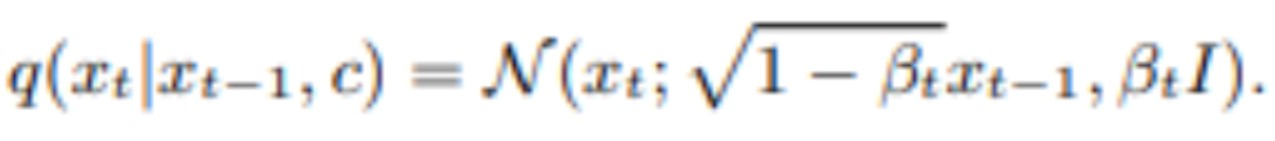
\includegraphics[width=.6\textwidth, keepaspectratio]{images/eq1.jpg}
    
    % \caption{فرایند diffusion}
    \label{fig:eq1}
\end{figure}

کل فرآیند انتشارq(x1:T∣x0,c)  یک فرآیند مارکوفی است و می‌تواند به صورت زیر تجزیه شود:

\begin{figure}[h]

    \centering
    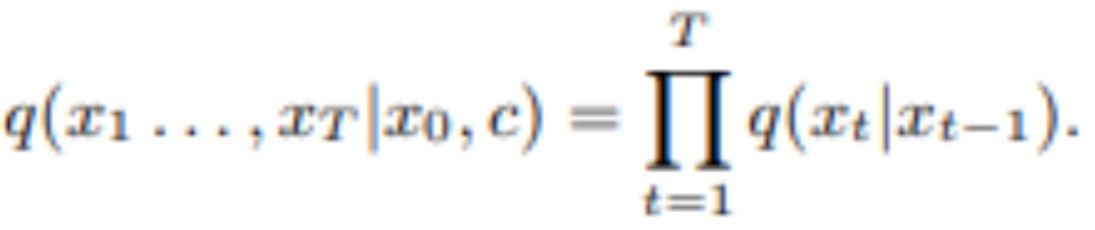
\includegraphics[width=.6\textwidth, keepaspectratio]{images/eq2.jpg}
    
    % \caption{فرایند diffusion}
    \label{fig:eq2}
\end{figure}

فرآیند معکوس یک روش تولید مل-اسپکتروگرام است که دقیقاً برخلاف فرآیند انتشار عمل می‌کند. برخلاف فرآیند انتشار، هدف فرآیند معکوس بازیابی یک مل-اسپکتروگرام از نویز گوسی است. فرآیند معکوس به عنوان توزیع شرطی pθ​(x0:T−1​∣xT​,c) تعریف می‌شود و می‌تواند بر اساس خاصیت زنجیره مارکوف به چندین انتقال تجزیه شود:

\begin{figure}[h]

    \centering
    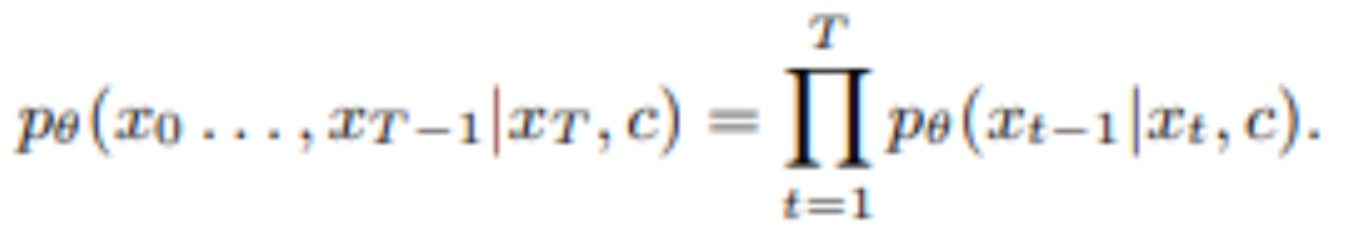
\includegraphics[width=.6\textwidth, keepaspectratio]{images/eq3.jpg}
    
    % \caption{فرایند diffusion}
    \label{fig:eq3}
\end{figure}

دیف-TTS شامل یک رمزگذار متن، رمزگذار مرحله، پیش‌بینی‌کننده مدت زمان، و رمزگشا است. 
شبکه رمزگشا شامل یک پشته از 12 بلوک مقاوم با Conv1D، tanh، sigmoid و کانولوشن‌های 1x1 با 512 کانال مقاوم است [29]. همان‌طور که در شکل 3 نشان داده شده است، تعبیه فونم توسط تنظیم‌کننده طول گسترش می‌یابد. سپس، تعبیه فونم و خروجی رمزگذار مرحله به ورودی پس از لایه Conv1D اضافه می‌شود. لایه Conv1D اندازه هسته‌ای برابر 3 بدون گشادگی دارد. پس از عبور از این بلوک مقاوم، خروجی‌ها قبل از پس-نت جمع می‌شوند. در نهایت، رمزگشا نویز گوسی متناظر با دنباله فونم و مرحله زمانی انتشار را به دست می‌آورد.

\begin{figure}[h]

    \centering
    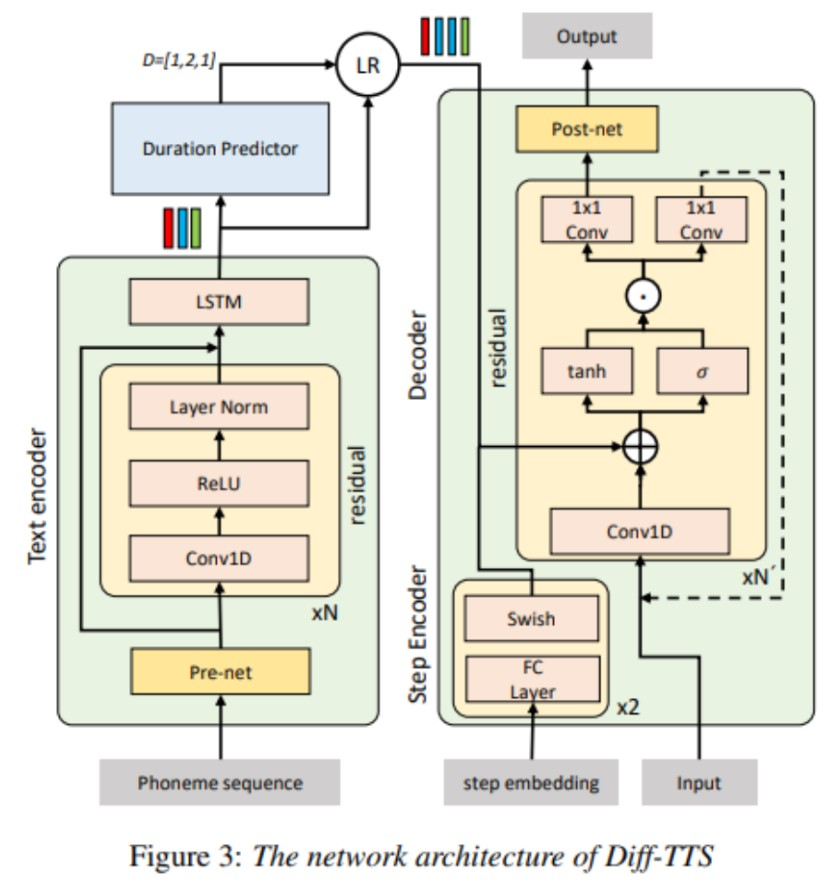
\includegraphics[width=.6\textwidth, keepaspectratio]{images/diff-tts.jpg}
    
    \caption{معماری diff-tts}
    \label{fig:diff-tts}
\end{figure}

\section{\lr{A Study on Speech Enhancement Based on Diffusion Probabilistic Model}}
مدل‌های احتمالاتی انتشار توانایی فوق‌العاده‌ای در مدل‌سازی تصاویر طبیعی و فرم‌های صوتی خام از طریق فرآیندهای جفت‌شده انتشار و معکوس نشان داده‌اند. ویژگی منحصر به فرد فرآیند معکوس (یعنی حذف سیگنال‌های غیرهدف از نویز گوسی و سیگنال‌های نویزی) می‌تواند برای بازیابی سیگنال‌های تمیز استفاده شود. بر اساس این ویژگی، ما مدل بهبود گفتار مبتنی بر مدل احتمالاتی انتشار (DiffuSE) را پیشنهاد می‌کنیم که هدف آن بازیابی سیگنال‌های گفتاری تمیز از سیگنال‌های نویزی است. معماری اساسی مدل DiffuSE پیشنهادی مشابه معماری DiffWave است—مدل تولید فرم صوتی با کیفیت بالا که هزینه محاسباتی و ردپای نسبتاً پایینی دارد. برای دستیابی به عملکرد بهتر در بهبود، ما فرآیند معکوس پیشرفته‌ای طراحی کردیم که به آن فرآیند معکوس حمایتی گفته می‌شود و در هر مرحله زمانی، گفتار نویزی را به گفتار پیش‌بینی‌شده اضافه می‌کند. نتایج تجربی نشان می‌دهد که DiffuSE عملکردی معادل با مدل‌های تولید صوت مرتبط در وظیفه SE مجموعه داده Voice Bank استاندارد شده دارد. علاوه بر این، نسبت به برنامه نمونه‌برداری کامل معمولاً پیشنهاد شده، فرآیند معکوس حمایتی پیشنهادی به ویژه سرعت نمونه‌برداری سریع را بهبود بخشیده و با انجام چندین مرحله نتایج بهبود بهتری نسبت به فرآیند استنتاج کامل سنتی ارائه می‌دهد.
در مدل پیشنهادی DiffuSE، ما یک فرآیند معکوس حمایتی جدید را استخراج می‌کنیم تا جایگزین فرآیند معکوس اصلی شود و سیگنال‌های نویز را به طور مؤثرتری از ورودی نویزی حذف کنیم.

در مدل احتمالی انتشار اصلی، نویز گوسی در فرآیند معکوس اعمال می‌شود. از آنجا که سیگنال گفتار تمیز در طول فرآیند معکوس دیده نمی‌شود، سیگنال گفتار محاسبه شده  xt​ ممکن است در طول فرآیند معکوس از مرحله T تا t+1 تحریف شود. برای حل این مشکل، ما فرآیند معکوس حمایتی را پیشنهاد دادیم، که فرآیند نمونه‌برداری را از سیگنال گفتار نویزی y آغاز می‌کند و y را در هر مرحله معکوس ترکیب می‌کند در حالی که سیگنال گوسی اضافی را کاهش می‌دهد.
شکل 2 ساختار مدل DiffuSE را نشان می‌دهد. همانند DiffWave، تنظیم‌کننده در DiffuSE هدفش حفظ شباهت سیگنال خروجی به سیگنال گفتار هدف است، که اجازه می‌دهد نویز و گفتار تمیز را از داده‌های مخلوط جدا کند. 

\begin{figure}[h]

    \centering
    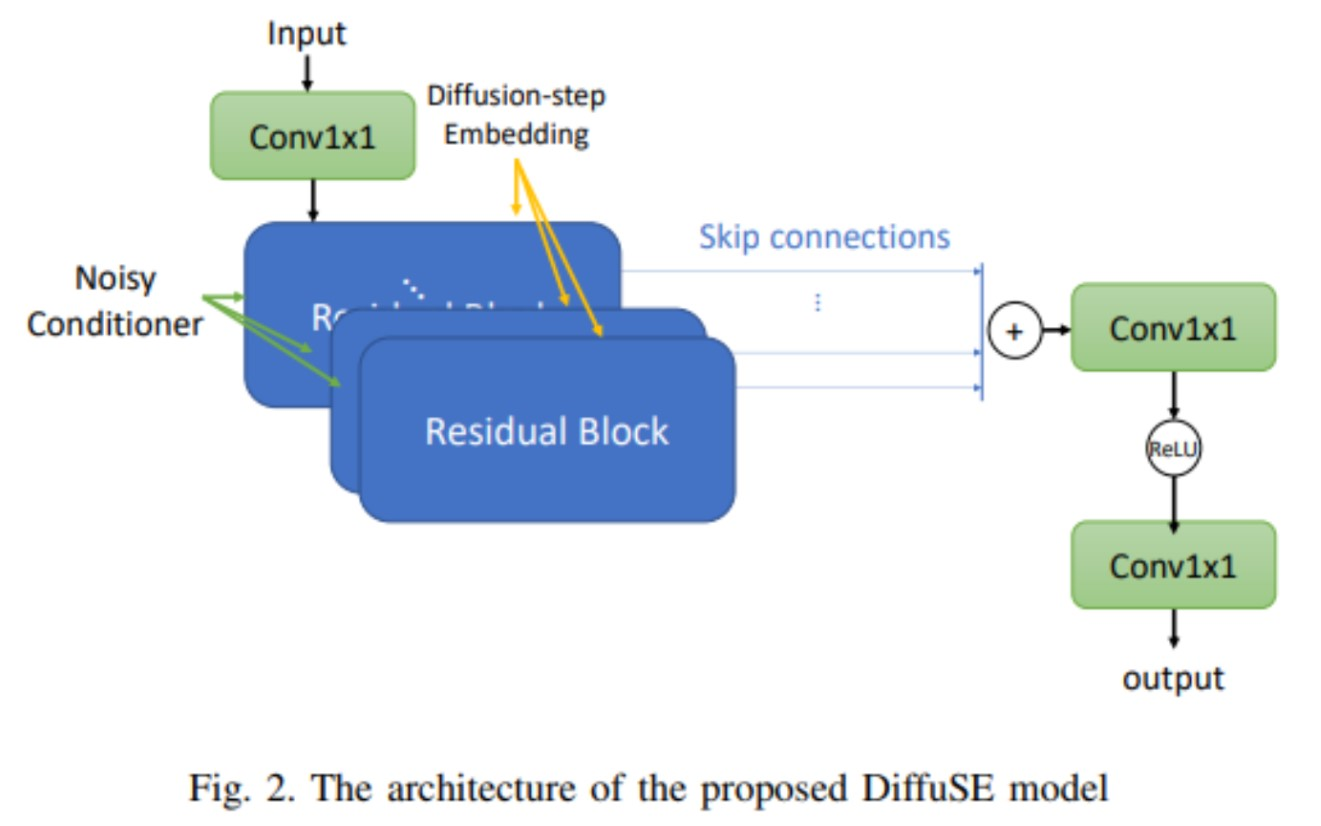
\includegraphics[width=.6\textwidth, keepaspectratio]{images/diffuSE.jpg}
    
    \caption{معماری diffuSE}
    \label{fig:diffuSE}
\end{figure}

برای تولید سیگنال‌های گفتار با کیفیت بالا، مدل DiffuSE را با ویژگی‌های Mel-spectral تمیز پیش‌آموزی کردیم. در DiffWave، اطلاعات شرطی مستقیماً از گفتار تمیز گرفته می‌شود که به مدل اجازه می‌دهد تا گفتار تمیز و نویز را از سیگنال‌های مخلوط جدا کند. پس از پیش‌آموزش، تنظیم‌کننده را از ویژگی‌های Mel-spectral تمیز به ویژگی‌های spectral نویزی تغییر دادیم، پارامترهای رمزگذار تنظیم‌کننده را مجدداً تنظیم کردیم و دیگر پارامترها را برای آموزش SE حفظ کردیم. در نهایت از نمونه‌برداری سریع استفاده شد تا تعداد مراحل حذف نویز کاهش پیدا کند.

\chapter{دادگان}
اگرچه دادگان انگلیسی میتوانند برای آموزش مدل پایه از صفر به کار آیند، لازم است که حداقل یک مرحله ی 
fine-tuning بر روی زبان فارسی انجام شود. طی جستجوهایی که انجام شد، دیتاست بزرگ و شناخته شدهای برای تسک  
 Speech Enhancement and Denoisingبرای زبان فارسی وجود ندارد. بنابراین نیاز است
  تا دیتاستی شامل جفت صوت های تمیز و نویزدار بسازیم. 
  ما در این پروژه دو رویکرد را در پیش گرفتیم و 
  نهایتا دو دیتاست synthesized و recorded را ارائه نمودیم.

\section{دیتاست synthesized}
در این بخش ما از صداهای validated بخش فارسی دیتاست CommonVoice استفاده کردیم.
به این ترتیب که تعدادی از این صداها را به عنوان صوت تمیز در نظر گرفتیم و سپس معادل نویزی آن‌ها را به صورت اتوماتیک تولید کردیم.
در این فرایند، هر صوت با احتمال یک‌دوم با یک نویز بک‌گراند از نویز gaussian ترکیب می‌شود و با 
احتمال یک‌دوم هم با یک صوت صدای بک‌گراند از نوع \lr{crowd talking}.
برای این اصوات، ما مجموعه‌ی کوچکی از فایل‌های صوتی \lr{crowd talking} را از pixabay جمع‌آوری کردیم و به صورت رندوم، هر بار یک مورد از آن‌ها را برگزیده و با صوت تمیز تلفیق کردیم.
نتیجه‌ی این بخش ۶۰۰۰ زوج صوت تمیز و نویزی سنتزشده می باشد که ۱۰۰۰ مورد از آن‌ها به عنوان مجموعه‌ی تست و ۵۰۰۰ مورد از آن‌ها به عنوان مجموعه‌ی train جدا شدند.
subset تست این دادگان در مخزن پروژه بارگزاری شده‌است.

\section{دیتاست recorded}  
در این بخش ما
 از یک مجموعه داده شامل صوت های تمیز فارسی استفاده کردیم 
و دقیقا همین اصوات را در محیط‌هایی با یک صدای بکگراند پخش کردیم و مجددا ضبط کردیم.
به این ترتیب هر دوی داده‌ی تمیز و نویزی شامل گفتار عینا یکسانی می‌شدند اما دیگر صدای بک‌گراند به صورت مصنوعی به داده اضافه نشده بود.
ایده‌ی اصلی این بود که تمام صدا‌های محیطی نیز کاملا طبیعی باشند. اما به علت محدودیت‌های موجود، بخشی از این نمونه‌ها با صدای طبیعی محیط (مانند صدای طبیعت یا فن) هستند و برخی دیگر با یک صدای آماده که در محیط پخش شده‌است.

برای دیتاست اصوات تمیز گزینه‌های زیادی از میان دیتاست‌ها وجود داشت. از جمله:

\begin{itemize}
    \item \href{https://www.kaggle.com/datasets/magnoliasis/persian-tts-dataset}{persian-tts-dataset}
    \item \href{https://www.kaggle.com/datasets/moradi/persian-texttospeech-audio}{persian-texttospeech-audio}
    \item \href{https://huggingface.co/datasets/Kamtera/ParsiGoo}{ParsiGoo}
    \item \href{https://fa.persianspeechcorpus.com/}{\lr{Persian SpeechCorpus}}
    \item \href{https://github.com/persiandataset/PersianSpeech}{PersianSpeech}
    \item \href{https://www.kaggle.com/datasets/amirpourmand/automatic-speech-recognition-farsi-youtube}{\lr{farsi ASR youtube}}
    \item \href{https://commonvoice.mozilla.org/en/datasets}{CommonVoice}
    \item \href{https://github.com/shenasa-ai/speech2text}{\lr{Shenasa ai}}
\end{itemize}

ما در این پروژه از صوت های دیتاست persian-tts-dataset به عنوان صوت های تمیز بدون نویز استفاده کردیم. برای ساختن صوت های نویز دار متناظر، از 5 صدای پس زمینه زیر استفاده کردیم:
\begin{itemize}
    \item صدای محیط (صدای طبیعی محیط) --> 5 صوت
    \item صدای فن (صدای طبیعی فن) --> 20 صوت
    \item صدای باران (ضبط شده آماده) --> 24 صوت
    \item صدای شهر (ضبط شده آماده) --> 25 صوت
    \item صدای جنگل (ضبط شده آماده) --> 18 صوت
    \item صدای تشویق ورزشگاه (ضبط شده آماده) --> 30 صوت
\end{itemize}

دو صدای نویز اول مربوط به صدای محیط و فن هستند که در این دو محیط قرار گرفته و صدای تمیز را پخش کرده و ضبط کردیم. برای 4 مورود دیگر که صداهای از قبل ضبط شده پس زمینه هستند، به طور همزمان صدای تمیز و نویز را اجرا کرده و صدا را ضبط کردیم تا صدای نویزدار را به دست آوریم. در نهایت توانستیم 122 جفت داده صدای تمیز و صدای نویزدار را به دست آوریم.
این دیتاست نیز در مخزن پروژه بارگزاری شده‌است و برای fine-tuning مورد استفاده قرار گرفته است.

\chapter{متدولوژی}
همانطور که در بخش مقدمه ذکر شد، ما دو رویکرد rule-based و رویکرد مبتنی بر شبکه‌های عصبی را در پیش گرفتیم که در ادامه شرح داده می‌شود.

\section{راهکار rule-based}
در این بخش از دو ابزار پایتونی به شرح زیر استفاده کردیم:
\begin{itemize}
    \item \textbf{کتاب خانه‌ی librosa:} در یک بخش از این ابزار، صدای ورودی بررسی می‌شود تا هر گونه موزیک بک‌گراندی از آن حذف شود و تنها گفتار باقی بماند. این تسک \lr{source separation} نیز نام دارد و در کتاب‌خانه‌ی librosa با کیفیت بالایی پیاده‌سازی شده‌است.
    \item \textbf{کتاب‌خانه‌ی noisereduce:} یکی دیگر از کتاب‌خانه‌های پایتون نیز برای حذف نویز‌های بی‌معنای بک‌گراند به کار می‌آیند. این کتابخانه noisereduce نام دارم و به عنوان بخش دوم ابزار rule-based ایفای نقش می‌کند.
\end{itemize}

این ابزار نیز همانند ابزار‌های مبتنی بر شبکه‌های عصبی مورد ارزیابی قرار گرفته و در chapter بعد نتایج آن ذکر می‌شود.

\section{راهکار مبتنی بر شبکه‌ی عصبی}
فعالیت ما در این بخش به دو فاز تقسیم می‌شود.
در فاز اولیه، ما تعداد زیادی از معماری‌های پیشین موجود را برای بررسی کیفیت و عملکر آن‌ها و اینکه آیا قابلیت بهبود دارند یا خیر آزمایش کردیم.
در فاز بعدی نیز در جهت بهبود سه مورد از بهترین این معماری‌ها کوشیدیم.

\susection{آزمون معماری‌های موجود}
معماری‌هایی که در پروپوزال پروژه معرفی شده‌بودند از قرار زیر هستند:

\begin{itemize}
    \item \href{https://github.com/speechbrain/speechbrain/tree/develop/recipes/Voicebank/enhance/MetricGAN}{speechbrain metricGAN}
    \item \href{https://github.com/nvidia/cleanunet}{CleanUnet}
    \item \href{https://github.com/keonlee9420/DiffSinger}{DiffSinger}
    \item \href{https://github.com/haoxiangsnr/FullSubNet}{FullSubNet}
    \item \href{https://github.com/resemble-ai/resemble-enhance}{resemble-enhance}
    \item \href{https://github.com/drethage/speech-denoising-wavenet}{speech-denoising-wavenet}
    \item \href{https://github.com/breizhn/DTLN}{DTLN}
\end{itemize}

ما در این فاز از پروژه، سعی کردیم بسیاری از این معماری‌ها و برخی که بعد از پروپوزال به آن‌ها رسیدیم آزمایش کنیم.
اول از این جهت که عملکرد آن‌ها روی گفتار فارسی چگونه است و دوم از این جهت که آیا می‌توان آن‌ها را به روش‌هایی چون training و fine-tuning برای زبان فارسی بهبود داد یا خیر.
معماری‌های بررسی شده در این بخش شامل 
MetricGAN نسخه‌ی speechbrain و MetricGAN نسخه‌ی مخزن \href{https://github.com/wooseok-shin/MetricGAN-plus-pytorch}{MetricGAN-plus-pytorch}
و 
دینویزر \href{https://github.com/microsoft/DNS-Challenge}{DNS-Challenge}
و 
معماری موفق resemble-enhance
و 
Clean-Unet
 و DTLN
 و 
 speech-denoising-wavenet
 و
 \href{https://github.com/facebookresearch/denoiser}{denoiser} 
 می‌شوند.
 نوتبوک مربوط به آزمایش این مدل‌ها در مخزن پروژه موجود است.
نهایتا در این بخش، سه مخزن 
زیر علاوه بر داشتن خروجی مناسب، برای آموزش یا fine-tuning نیز مناسب تشخیص داده شدند.

\begin{itemize}
    \item https://github.com/wooseok-shin/MetricGAN-plus-pytorch
    \item https://github.com/speechbrain/speechbrain/recipes/Voicebank/enhance/MetricGAN
    \item https://github.com/resemble-ai/resemble-enhance
\end{itemize}

\susection{بهبود معماری‌های موجود}
در این بخش ما سه معماری ذکر شده را train یا fine-tune کردیم که شرح آن در ادامه می‌آید.

\paragraph{MetricGAN-plus-pytorch}
از آن‌جا که مدل pre-trained ارائه شده توسط این معماری قابلیت fine-tuning را نداشت، ما مدل را از ابتدا روی دیتاست VCTK آموزش دادیم.
این مدل به تعداد ۷۵۰ ایپاک و به مدت حدود ۲ روز آموزش دید و مدل نهایی آن به همراه log های آموزش آن در مخزن پروژه بارگزاری گردیده‌است.
اما متاسفانه مدل خروجی performance خوبی بر روی دادگان تست نداشت. بنابراین به سراغ مدل MetricGAN ای که در قالب framework پرکاربرد speechbrain ارائه شده بود رفتیم.


\paragraph{MetricGAN-speechbrain}
ما این مدل را نیز که نیازمند ورژن دیگری از دیتاست VCTK بود ستاپ کردیم و به مدت حدود ۲ روز و به همان تعداد ایپاک آموزش دادیم.
نوتبوک مربوط به ستاپ و اسکرین‌شاتی از مراحل نهایی آموزش آن در مخزن پروژه بارگزاری شده‌است.
این مدل عملکرد بهتری نسبت به مدل قبل داشت اما همچنان performance آن به نسبت مدل pre-trained ای که خودشان روی مخزن پروژه قرار داده بودند inferior بود.
بنابراین ما هم در این ورژن را به مدل حاصله ترجیح دادیم و به عوان مدل core در application خود آن را Embed کردیم.

در یک تلاش دیگر، ما این مدل را برای fine-tuning ستاپ کردیم و این بار به کمک داده‌هایی که خودمان record کرده بودیم، به تعداد ایپاک کمی با یک learning-rate کوچک مناسب برای fine-tuning آن را آموزش دادیم.
خروجی‌های این مدل از دو مورد قبل بهتر بودند و در بخش ارزیابی مورد بررسی قرار می‌گیرند.
مدل fine-tune شده در این بخش به همراه script های آموزش آن نیز در مخزن پروژه قرار دارند.


\paragraph{resemble-enhance} 
در انتها با توجه به خروجی‌های بسیار با کیفیت resemble-enhance تصمیم گرفتیم که این مدل را نیز بر روی دادگان فارسی خود آموزش دهیم تا نتیجه را مقایسه کنیم.
در مخزن پروژه، یک نوتبوک نیز به این امر اختصاص داده شده و نتایج آن در بخش‌های بعدی خواهد آمد.


\chapter{application آزمون مدل منتخب}
در بخشی از این پروژه ما یک اپلیکیشن ساده بر بستر PyQt ایجاد کردیم که می‌تواند برای بررسی خروجی مدل منتخب بر روی صدا‌های نویزی مورد استفاده قرار بگیرد.
این اپلیکیشن مینیمال، برای بارگذاری، بهبود و شنیدن صدای بهبود یافته مانند شکل زیر طراحی شده‌است.

\begin{figure}[h]

    \centering
    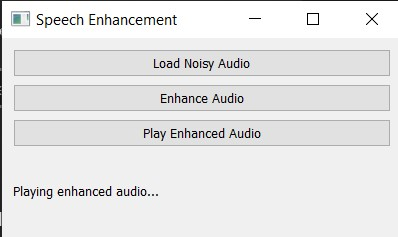
\includegraphics[width=.6\textwidth, keepaspectratio]{images/app.jpg}
    
    \caption{\lr{testing application}}
    \label{fig:app}
\end{figure}

برای راه اندازی این اپلیکیشن روی device خود کافی است requirement های موجود در requirements.txt را نصب کنید و دستور \lr{Py app.py} را اجرا کنید.
همچنین اگر سیستم شما ویندوز است، لازم است تنظیمات خود را به صورت تصویر زیر تغییر دهید.

\begin{figure}[h]

    \centering
    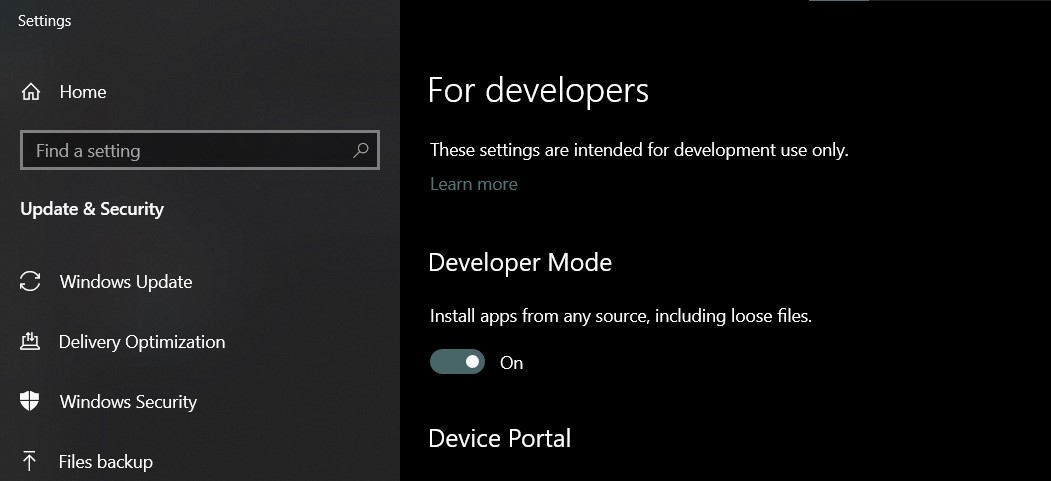
\includegraphics[width=.6\textwidth, keepaspectratio]{images/setting.jpg}
    
    \caption{\lr{windows app settings}}
    \label{fig:setting}
\end{figure}

\end{document}
